\begin{frame}{Feature Branches}
\begin{columns}[T]
  \begin{column}{.45\textwidth}
    \begin{block}{}
      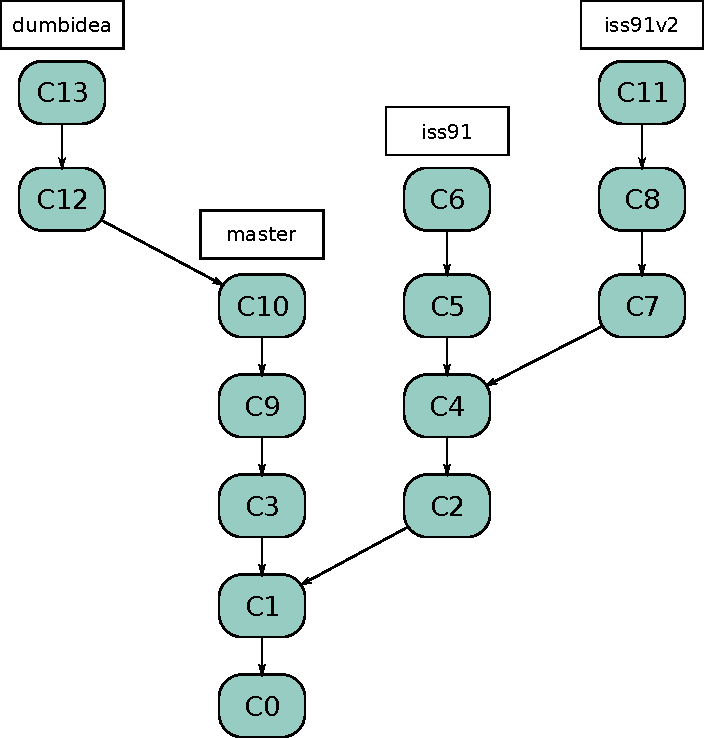
\includegraphics[scale=0.4]{images/feature-branches1.pdf}
    \end{block}
  \end{column}
  \begin{column}{.1\textwidth}
    \begin{block}{}
      \pause $\longrightarrow$
    \end{block}
  \end{column}
  \begin{column}{.45\textwidth}
    \begin{block}{} 
        \pause 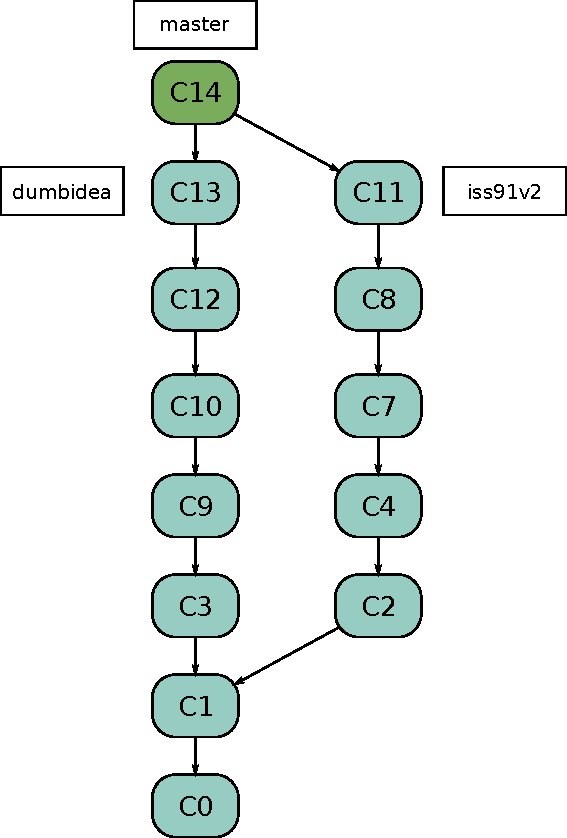
\includegraphics[scale=0.4]{images/feature-branches2.pdf}
    \end{block}
  \end{column}
\end{columns}  
\begin{tiny}
\pause \texttt{git merge dumbidea} \\
\pause \texttt{git merge iss91v2} \\
\pause \texttt{git branch -D iss91} \\
\end{tiny}
\end{frame}

\begin{frame}{Long-Running Branches}
  \begin{figure}
  \centering
    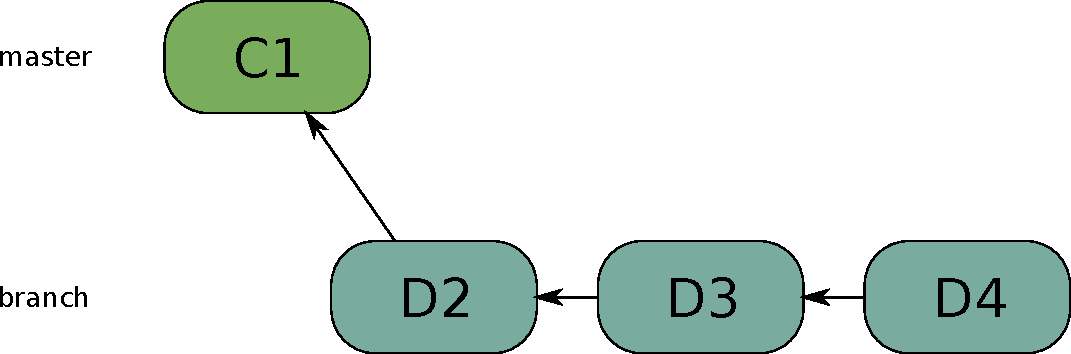
\includegraphics[scale=0.5]{images/long-running-branch.pdf}
  \end{figure}
  \tiny
  \begin{itemize}
  \pause \item \texttt{git checkout -b branch}
    \begin{itemize}
	  \pause \item \tiny \texttt{ändere Datei}
	  \pause \item \texttt{git add Datei}
	  \pause \item \texttt{git commit}
    \end{itemize}
  \end{itemize}
\end{frame}


\begin{frame}{Long-Running Branches}
  \begin{figure} 
  \centering
    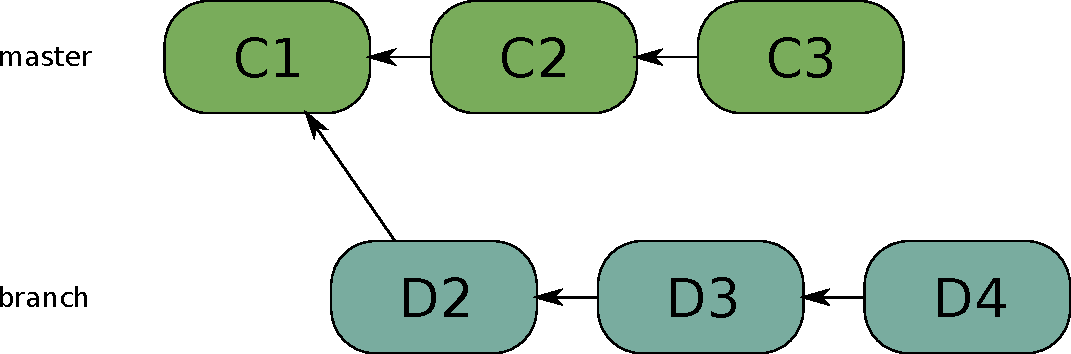
\includegraphics[scale=0.5]{images/long-running-branch2.pdf}
  \end{figure}
  \tiny
  \begin{itemize}
    \pause \item \texttt{git checkout master}
    \begin{itemize}
      \pause \item \tiny \texttt{ändere "file"}
      \pause \item \texttt{git add file} 
      \pause \item \texttt{git commit}
    \end{itemize}
  \end{itemize}
\end{frame}

\begin{frame}{Long-Running Branches}
  \begin{figure} 
  \centering
    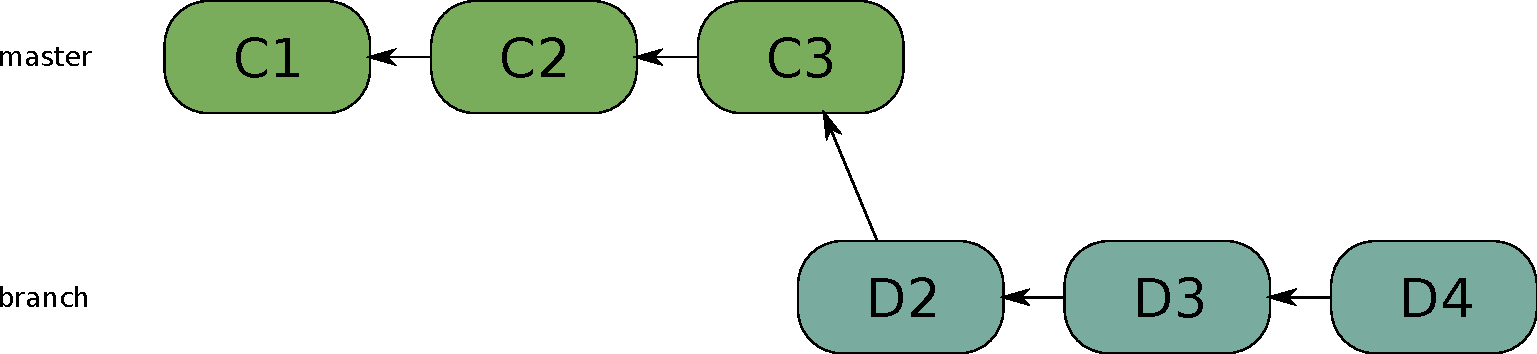
\includegraphics[scale=0.4]{images/long-running-branch3.pdf}
  \end{figure}
  \tiny
  \begin{itemize}
    \pause \item \texttt{git checkout branch}
    \pause \item \texttt{git rebase master}
  \end{itemize}
\end{frame}

%\begin{frame}{Merge Konflikte}
%  bla
%\end{frame}

\begin{frame}{Zentralisierter Workflow}
  \begin{figure} 
  \centering
    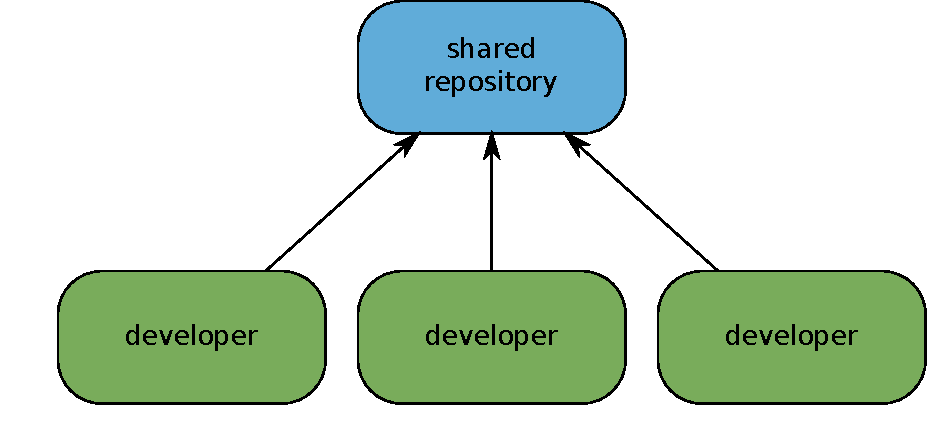
\includegraphics[scale=0.6]{images/centralized/centralized-workflow.pdf}
  \end{figure}
  \begin{itemize}
    \pause \item Bekannt aus SVN
    \pause \item Git verhindert überschreiben von Daten
  \end{itemize}
\end{frame}

\begin{frame}{Zentralisierter Workflow (Kommandos)}
\begin{columns}[T]
  \begin{column}{.5\textwidth}
    \begin{block}{}  
		\includegraphics<1>[scale=0.4]{images/centralized/centralized-workflow-clone.pdf}
		\includegraphics<2>[scale=0.4]{images/centralized/centralized-workflow-work.pdf}
		\includegraphics<3>[scale=0.4]{images/centralized/centralized-workflow-conflict.pdf}
		\includegraphics<4>[scale=0.4]{images/centralized/centralized-workflow-clone.pdf}
		\includegraphics<5>[scale=0.4]{images/centralized/centralized-workflow-push.pdf}
    \end{block}
  \end{column}
  \begin{column}{.5\textwidth}
    \begin{block}{}
    	\begin{tiny}
		\begin{itemize}
		  \item \texttt{git clone <repository>}
  		  \pause \item change "file"
		  \item \texttt{git add <file>}
  		  \item \texttt{git commit [-m"message"]}
  		  \pause
		  \pause \item \texttt{[git pull]}
  		  \pause \item \texttt{git push}
		\end{itemize}
    	\end{tiny}		
    \end{block}
  \end{column}
\end{columns}  
\end{frame}

\begin{frame}{Zentralisierter Workflow (Branching)}
\begin{columns}[T]
  \begin{column}{.5\textwidth}
    \begin{block}{}  
		\includegraphics<1>[scale=0.4]{images/centralized/centralized-workflow-branch-clone.pdf}
		\includegraphics<2>[scale=0.4]{images/centralized/centralized-workflow-branch.pdf}
		\includegraphics<3>[scale=0.4]{images/centralized/centralized-workflow-branch-master.pdf}
		\includegraphics<4>[scale=0.4]{images/centralized/centralized-workflow-branch-merge.pdf}
		\includegraphics<5>[scale=0.4]{images/centralized/centralized-workflow-branch-push.pdf}
    \end{block}
  \end{column}
  \begin{column}{.5\textwidth}
    \begin{block}{}
    	\begin{tiny}
		\begin{itemize}
		  \item \texttt{git clone <repository>}
  		  \pause \item \texttt{git checkout [-b] jira198}
		  \item \texttt{change "file"}
  		  \item \texttt{git add <file>}
  		  \item \texttt{git commit [-m"message"]}
  		  \pause \item \texttt{git checkout master}
   		  \pause \item \texttt{git merge jira198}
  		  \pause \item \texttt{git push}
		\end{itemize}
    	\end{tiny}		
    \end{block}
  \end{column}
\end{columns}  
\end{frame}

\begin{frame}{Integration-Manager Workflow}
  \begin{figure} 
  \centering
    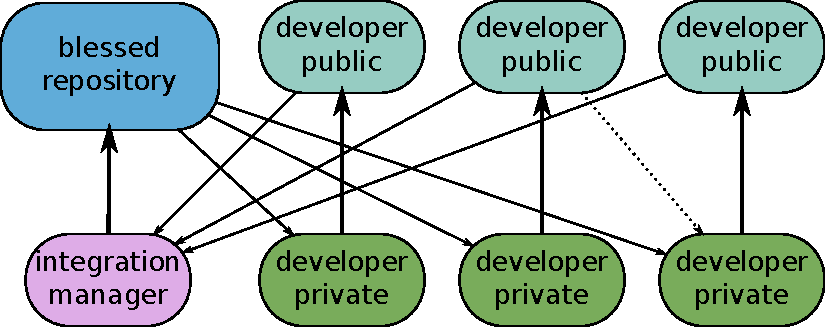
\includegraphics[scale=0.6]{images/integration-manager-workflow.pdf}
  \end{figure}
  \begin{itemize}
    \pause \item The project maintainer pushes to their public repository.
    \pause \item A contributor clones that repository and makes changes.
    \pause \item The contributor pushes to their own public copy.
    \pause \item The contributor sends the maintainer an e-mail asking them to pull changes.
    \pause \item The maintainer adds the contributor’s repo as a remote and merges locally.
    \pause \item The maintainer pushes merged changes to the main repository.
  \end{itemize}
\end{frame}

\begin{frame}{Dictator and Lieutenant Workflow}
  \begin{figure} 
  \centering
    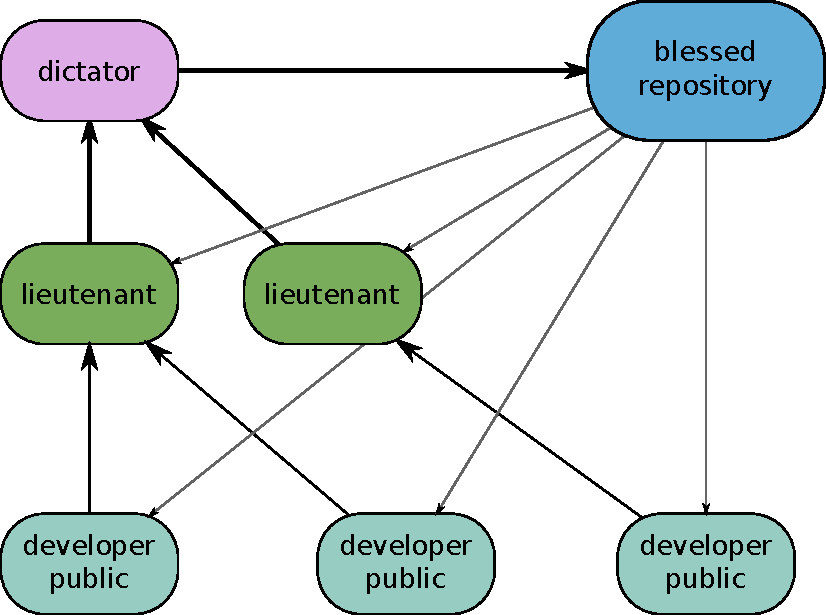
\includegraphics[scale=0.3]{images/dictator-and-lieteutnant-workflow.pdf}
  \end{figure}    
  \begin{itemize}
    \pause \item Regular developers work on their topic branch and rebase their work on top of master. The master branch is that of the dictator.
    \pause \item Lieutenants merge the developers’ topic branches into their master branch.
    \pause \item The dictator merges the lieutenants’ master branches into the dictator’s master branch.
    \pause \item The dictator pushes their master to the reference repository so the other developers can rebase on it.
  \end{itemize}
\end{frame}
